
\section{Burning}\label{sec:burning}

I have had the fantastic opportunity of working with scientists all over the world during this PhD project. I owe thanks for these opportunities to our wide network of collaborators as well as the EtiteForsk Travel Grant that I was awarded by the Danish Ministry for Higher Education and Science in 2018. (I have been especially quick to take opportunities to travel to the United States, since I also visited friends and family on those trips.)

Figure \ref{fig:flying} shows the institutes that I have visited and conferences that I have attended during the three years of my PhD on a map of the world. The routes that I have flown are shown together with their distance and the number of times that I flew that route.

While grateful for all of these opportunites, I am not proud of how much I have been traveling, and plan on much less air travel in the future. Each trip has come with an environmental cost, since air travel is the most \ch{CO2}-intensive activity an individual can choose to do.

\begin{figure}[b!]
	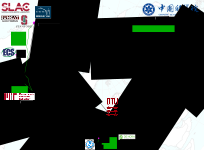
\includegraphics[width=\textwidth]{05_Impact/fig/flying.png}
	\caption{Map of research collaborations, conferences, and flights during this PhD project, superimposed on a map of the northern hemisphere. Flights are indicated as black lines, and the distance and total number of one-way flights I took over the three-year period September 2016-August 2019 are indicated. The projects requiring the most traveling have been beamline experiments at SLAC in California (Paper \ref{Scott2019_GIXRD}) and the collaboration with the Chinese Academy of Sciences (CAS) in Fuzhou, Fujian, China.}
	\label{fig:flying}
\end{figure}

Adding up all of the trips in Figure \ref{fig:flying}, I have flown 187600 km during this PhD project, equivalent to circling the earth 4.7 times at the equator. Using an average greenhouse gas emissions of 0.19 kg \ch{CO2} equivalents per passenger per kilometer\cite{Larsson2018}, this is 36 tons of \ch{CO2}, or 12 tons of \ch{CO2} per year (3.2 tC/yr). This is actually a slight underestimation, since it uses the direct-flight distances, whereas most of the trips indicated involved at least one transfer.

Domestic \ch{CO2} emissions per capita in Denmark in 2017 were 6.1 tons of \ch{CO2} per year\cite{Ritchie2019a} (1.7 tC/yr), so the flying alone during my PhD project represents approximately twice the average person's \ch{CO2} emissions in Denmark during the same period. 

There are numerous sources of \ch{CO2} emissions associated with the lab work of my PhD project. The only one considered here, which I believe to be the most significant, is that associated with electricity usage. The carbon footprint of equipment, chemicals, water, and consumables, for example, is not considered. Building 312 at DTU houses approximately 12 vacuum setups in active use including the EC-MS setup, which was the primary tool of my PhD project. The setup includes two roughing pumps, two turbo pumps, a large electronics rack, three computers and a number of control elements, and is left on 24 hours a day, 7 days a week. Others have used the EC-MS setup, and I have also used other setups, so taking responsibility for 1/12 of the hall's \ch{CO2} emissions seems a fair average. The heating (771 MWh) + electricity (162 MWh) used by building 312 in 2017 was 933 MWh. The carbon intensity of electricity generation in Denmark in 2017 was 291 kg \ch{CO2} per MWh of electricity\cite{DanishEnergyAgency}. Extrapolating to the 3-year PhD project, the \ch{CO2} cost of my lab work has been:
\begin{equation}
3 \text{[yr]} \cdot \frac{1}{12} \cdot 291 \left[\frac{\text{kg}_{\ch{CO2}}}{\text{MWh}}\right] \cdot 933\text{[MWh]} = 68 [\text{t}_{\ch{CO2}}]\,,
\end{equation}
which is 22.6 tons of \ch{CO2} per year (6.2tC/yr). This is a slight overestimation as I have assumed that the carbon intensity of heat is equal to that of electricity, when actually it is lower \cite{EnergiNet}. 

The \ch{CO2} cost of running the EC-MS setup is thus, surprisingly, even higher than the \ch{CO2} cost of the flying I have done during my PhD project. This would likely not be the case in the future, as progress in decarbonizing electricity is much faster than progress in decarbonizing aviation (see Chapter \ref{ch:Intro}). 

Adding the costs up my setup, travel, and living as an average Dane (probably an overestimation, as I have a vegetarian cyclist lifestyle when not traveling), the \ch{CO2} cost of my 3-year PhD project is approximately:
\begin{equation}
c = c_\text{el} + c_\text{travel} + c_\text{live} = 68 [\text{t}_{\ch{CO2}}] + 36 [\text{t}_{\ch{CO2}}] + 3 \text{[yr]} \cdot 6.1  [\text{t}_{\ch{CO2}}/\text{yr}] = 122 [\text{t}_{\ch{CO2}}]\label{eq:costs}
\end{equation}
That is the debt I have to pay, before I can even begin to claim that I'm helping to solve the climate crisis.


